%\documentclass[numsec,webpdf,modern,large,numbered]{oup-authoring-template}
\documentclass[numsec,webpdf,modern,large]{oup-authoring-template}

\graphicspath{{fig/}}

\usepackage{graphicx}
\usepackage{orcidlink}
\usepackage{hyperref}
\hypersetup{hidelinks}

\begin{document}

\journaltitle{Bioinformatics}
\DOI{DOI added during production}
\copyrightyear{YEAR}
\pubyear{YEAR}
\vol{XX}
\issue{x}
\access{Published: Date added during production}
\appnotes{Application Note}

\title[TomatoPromoterDesigner]{TomatoPromoterDesigner: a reproducible framework for motif-aware analysis and design of tissue-biased tomato promoters}

\author[1,2,3]{Zhoujie Fan}
\author[1,2]{Haimeng Zhang}
\author[1,2]{Xiaoyu Wang}
\author[1]{Hao Meng}
\author[1,3]{Hong Liang}
\author[4,5]{Zheng Wang}
\author[6]{Huazhu Fu\ORCID{0000-0002-9702-5524}}
\author[7]{Ching-Yu Cheng}
\author[1,2,3,8,*]{Shan Cong\ORCID{0000-0002-5981-7678}}
\author[1,2,3,7,*]{Xiaohui Yao\ORCID{0000-0002-8530-7989}}

\address[1]{\orgdiv{College of Intelligent Systems Science and Engineering}, \orgname{Harbin Engineering University}, \orgaddress{\street{Harbin}, \postcode{150001}, \country{China}}}
\address[2]{\orgdiv{Qingdao Innovation and Development Center}, \orgname{Harbin Engineering University}, \orgaddress{\street{Qingdao}, \postcode{266000}, \country{China}}}
\address[3]{\orgname{Sanya Nanhai Innovation and Development Base of Harbin Engineering University}, \orgaddress{\street{Sanya}, \postcode{572024}, \country{China}}}
\address[4]{\orgdiv{School of Psychological and Cognitive Sciences}, \orgname{Peking University}, \orgaddress{\street{Beijing}, \postcode{100871}, \country{China}}}
\address[5]{\orgdiv{School of Biomedical Engineering}, \orgname{Hainan University}, \orgaddress{\street{Sanya}, \postcode{572025}, \country{China}}}
\address[6]{\orgdiv{Institute for Infocomm Research}, \orgname{Agency for Science, Technology and Research}, \orgaddress{\street{Singapore}, \postcode{138632}, \country{Singapore}}}
\address[7]{\orgdiv{Department of Ophthalmology, Yong Loo Lin School of Medicine}, \orgname{National University of Singapore}, \orgaddress{\street{Singapore}, \postcode{119228}, \country{Singapore}}}
\address[8]{\orgdiv{Stem Cell and Regenerative Biology, Genome Institute of Singapore}, \orgname{A*STAR}, \orgaddress{\street{Singapore}, \postcode{138672}, \country{Singapore}}}

\corresp[*]{Corresponding authors. Xiaohui Yao (\href{mailto:xiaohui.yao@hrbeu.edu.cn}{xiaohui.yao@hrbeu.edu.cn}); Shan Cong (\href{mailto:shan.cong@hrbeu.edu.cn}{shan.cong@hrbeu.edu.cn})}

\received{Day}{Month}{Year}
\revised{Day}{Month}{Year}
\accepted{Day}{Month}{Year}

\abstract{
\textbf{Summary:} Engineering tissue-biased promoters in tomato requires computational approaches that connect regulatory sequence interpretation with promoter activity scoring and candidate design, but these tasks are often addressed by separate resources. TomatoPromoterDesigner is a reproducible Python framework that unifies promoter sequence processing, motif analysis, tissue-associated scoring and motif-aware promoter design within a single workflow. The framework integrates package-native modules with bundled model-backed routes, and provides standardized reporting and reproducible example workflows to support tomato promoter engineering studies.\\
\textbf{Availability and Implementation:} TomatoPromoterDesigner is implemented in Python and distributed as an installable command-line package. Source code, documentation and example workflows are freely available under the MIT license at \url{https://github.com/Yaolab-fantastic/TomatoPromoterDesigner}.\\
\textbf{Contact:} \href{mailto:xiaohui.yao@hrbeu.edu.cn}{xiaohui.yao@hrbeu.edu.cn}; \href{mailto:shan.cong@hrbeu.edu.cn}{shan.cong@hrbeu.edu.cn}.\\
\textbf{Supplementary information:} Supplementary data are available at \textit{Bioinformatics} online.
}

\keywords{tomato promoter engineering, tissue-biased expression, motif-aware design, reproducible workflow, synthetic biology}

\maketitle

\section{Introduction}

Precise regulation of gene expression is essential for plant synthetic biology and crop engineering, where tissue-biased promoters provide a means to control transgene activity with improved spatial specificity \citep{Peremarti2010,Amack2020}. Computational approaches can facilitate promoter engineering by enabling regulatory sequence interpretation, activity scoring, and candidate sequence design \citep{Kotopka2020,Cazier2021}. However, these capabilities are frequently implemented as separate tools or task-specific workflows, limiting their integration into reproducible promoter engineering pipelines.

Recent advances in regulatory sequence modeling have enabled diverse computational strategies for promoter analysis, including motif-based interpretation \citep{Lescot2002,Sandelin2004,Fornes2020}, promoter activity modeling \citep{Avsec2021,Washburn2019}, and sequence generation or optimization \citep{Yang2021}. Nevertheless, researchers often need to combine heterogeneous software components, input formats, and analysis procedures when moving from promoter characterization to candidate design. This fragmentation creates practical challenges for reproducibility, software accessibility, and systematic evaluation of computationally designed promoter candidates, particularly in crop-specific applications such as tomato promoter engineering \citep{Sato2012}.

Here, we present TomatoPromoterDesigner, a reproducible Python framework for motif-aware analysis and design of tissue-biased tomato promoters. The framework integrates promoter sequence processing, motif analysis, tissue-associated scoring, bundled model-backed routes, and candidate design within a unified workflow. TomatoPromoterDesigner provides an installable command-line interface, standardized reporting, visualization support, and reproducible example workflows. Its main contribution is to turn the project training code, model resources, sequence-processing logic and design utilities into a single inspectable software environment with documented input and output schemas. By connecting promoter interpretation, scoring, and design in one toolkit, TomatoPromoterDesigner provides a practical computational resource for reproducible tomato promoter engineering workflows.

\begin{figure}[t]
\centering
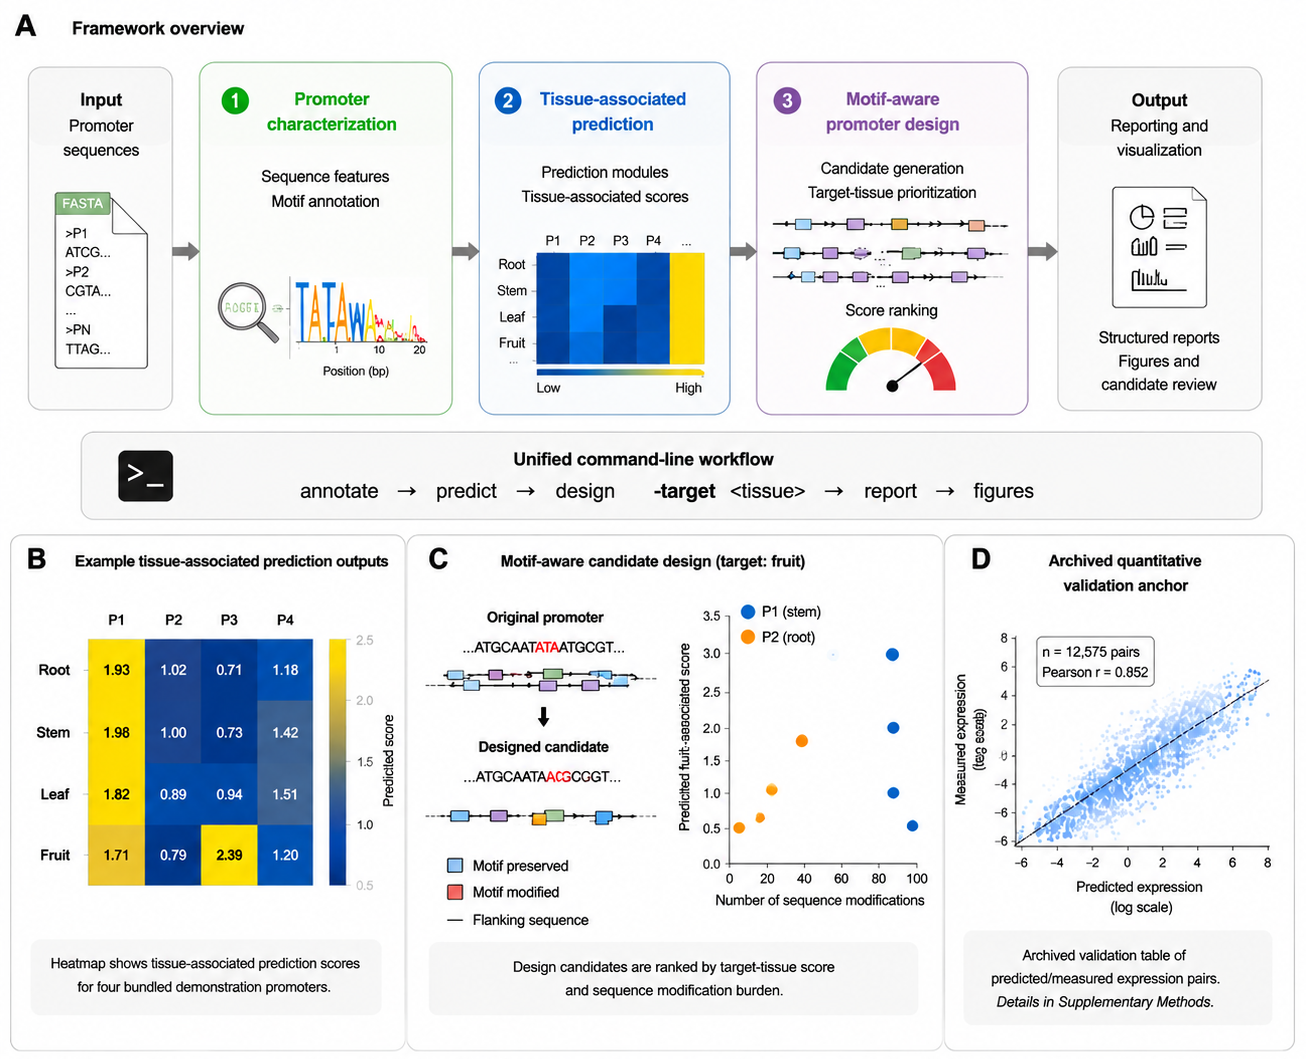
\includegraphics[width=\textwidth]{Framework.png}
\caption{Overview of TomatoPromoterDesigner. (A) The framework accepts one or more tomato promoter sequences, performs sequence validation and normalization, annotates regulatory motifs, generates tissue-associated scores, and connects these outputs to motif-aware candidate design and structured reporting. (B) Example four-tissue scoring output illustrates the common result schema used for root, stem, leaf and fruit-associated promoter prioritization. (C) The design workflow starts from an input promoter and a user-specified target tissue, then generates candidate sequences that can be compared with the original promoter using tissue-associated scores, sequence modification summaries and quality-control information. (D) Repository-retained quantitative resources and source tables support manuscript-facing reproducibility checks and supplementary figure reconstruction without presenting the current release as a large-scale model benchmark.}
\label{fig:framework}
\end{figure}

\section{Implementation}

TomatoPromoterDesigner is implemented as a modular Python framework for promoter analysis and design, with an emphasis on reproducibility, workflow consistency and command-line accessibility. The software is distributed as an installable package and exposes a unified command-line interface for sequence validation, motif annotation, tissue-associated scoring, candidate promoter design, report generation and figure export. This organization allows users to execute individual modules independently or combine them into an end-to-end workflow from promoter characterization to candidate evaluation.

The framework accepts standard sequence and tabular inputs and performs sequence validation, normalization and structured output generation to support reproducible downstream analysis. Promoter interpretation is supported through motif-analysis components that annotate regulatory sequence features and summarize motif-related outputs in standardized tables \citep{Lescot2002,Fornes2020}. The current release provides package-native motif scanning together with project-derived DNABERT motif post-processing \citep{Ji2021}, providing a stable interface for promoter interpretation while preserving compatibility with bundled model resources and retained tabular outputs.

For promoter prioritization, the framework provides a package-native deterministic operational scorer, a project-trained four-tissue VAE adapter informed by MpraVAE methodology \citep{Jin2024}, and a scalar-expression adapter based on the DeepSEED predictor \citep{Zhang2023}. The package-native and MpraVAE four-tissue routes use common tissue-score field names, whereas the DeepSEED route reports backend-labeled scalar outputs. Score definitions remain route-specific, and values from different backends are not assumed to share a calibrated numerical scale. This separation between interface and backend supports reproducible current use while allowing integration of additional validated scoring backends.

A central function of TomatoPromoterDesigner is motif-aware promoter design. Given an input promoter sequence and a target tissue, the design workflow generates candidate promoter sequences and evaluates them within the same reporting structure used for scoring outputs \citep{Yang2021,Cazier2021}. In the package-native route, candidate generation is performed through deterministic motif-aware sequence editing strategies, whereas the bundled MpraVAE route exposes latent-space design through an explicit checkpoint-backed command. Candidate outputs can be summarized with tissue-associated scores and quality-control information, enabling consistent comparison of original and designed promoter sequences for downstream review or experimental testing.

To support reproducible use, the framework includes structured reporting, lightweight visualization utilities, bundled example inputs, model checkpoints, source tables and provenance-aware data organization. The release wheel includes the checkpoints and model definitions required by the explicit model-backed scoring commands. Selected support tables, processed intermediate files and demonstration outputs are provided with the repository, whereas large optional resources are tracked separately through manifests and provenance documentation. Together, these features position TomatoPromoterDesigner as a practical computational framework for reproducible tomato promoter engineering workflows.

\section{Application Example and Reproducibility}

TomatoPromoterDesigner was evaluated as a reproducible workflow for processing, characterizing and designing tomato promoter sequences. The aim of this evaluation was not to establish a large-scale machine-learning benchmark, but to assess whether the framework could consistently connect promoter interpretation, tissue-associated scoring and candidate design within a unified software environment. Accordingly, we evaluated bundled tomato promoter examples distributed with the software release together with repository-retained quantitative tables generated during the project modeling workflow.

Using promoter examples bundled with the software package, TomatoPromoterDesigner generated standardized motif annotation outputs, tissue-associated score summaries, candidate design results and compact reports from the same input sequences. This workflow demonstrated that promoter sequence interpretation, scoring and design could be executed through a consistent command-line interface without manual conversion between intermediate formats. Motif-analysis outputs provided structured regulatory feature summaries, while the package-native scorer generated deterministic tissue-associated scores defined by the current release. The resulting design outputs connected candidate generation with downstream evaluation by summarizing scores, sequence modification information and quality-control indicators within a unified result schema. Together, these package-bundled examples illustrate the intended use of TomatoPromoterDesigner as an integrated promoter engineering workflow rather than a collection of independent analysis utilities.

As a repository-level reproducibility check, TomatoPromoterDesigner also retains source tables used to reconstruct the supplementary quantitative, motif, k-mer and design-summary figures. These resources are used to verify that manuscript-facing summaries can be regenerated from distributed tabular files and documented scripts. Detailed statistics, including the retained scalar-expression correlation analysis, are provided in the Supplementary Methods rather than presented as an independent benchmark of the current scoring components.

We further applied the design workflow to illustrate motif-aware promoter engineering in a tissue-targeted setting. Starting from an input tomato promoter sequence and a specified target tissue, TomatoPromoterDesigner generated candidate sequences together with tissue-associated scores, sequence modification summaries and quality-control information. In package-native routes, candidate generation is performed through deterministic motif-aware sequence editing, whereas the bundled MpraVAE design command supports checkpoint-backed latent-space candidate generation. This design stage connects sequence modification with downstream evaluation, allowing original and designed promoter candidates to be compared within a unified output structure and prioritized for subsequent manual review or experimental testing.

Together, these analyses demonstrate that TomatoPromoterDesigner provides a coherent software framework for tomato promoter engineering by linking promoter characterization, scoring, evaluation and candidate design through shared computational interfaces. The combination of reproducible example workflows, repository-retained project resources and structured reporting enables transparent inspection and extension of computational promoter design processes for downstream studies.

\section{Conclusion}

TomatoPromoterDesigner provides a reproducible computational framework that connects promoter sequence interpretation, tissue-associated scoring and motif-aware candidate design within a unified workflow for tomato promoter engineering. By combining modular software components, bundled model resources, structured reporting and provenance-aware resources, the framework enables transparent inspection and reproducible reuse of computational promoter analysis and design procedures. TomatoPromoterDesigner is intended to support researchers in prioritizing promoter candidates and integrating computational workflows into downstream experimental studies.

\bibliographystyle{oup-abbrvnat}
\bibliography{application_note_references}


\end{document}
